\chapter*{Annexes }
\addcontentsline{toc}{chapter}{Annexes}
\markboth{Annexes}{}
\stepcounter{chapter}
\addtocontents{lot}{\vspace{3.8mm}}
\addtocontents{lof}{\vspace{3.8mm}}

%Mettez vos annexes ici...

%===================== ANNEXE 1 =====================%
\section{Annexe 1: Complément des diagrammes de modélisation}
\subsection{Diagramme de cas d'utilisation global}
\addcontentsline{lof}{figure}{Annexe 1.1 Diagramme de cas d'utilisation global}
\begin{figure}[H]
    \centering
    \frame{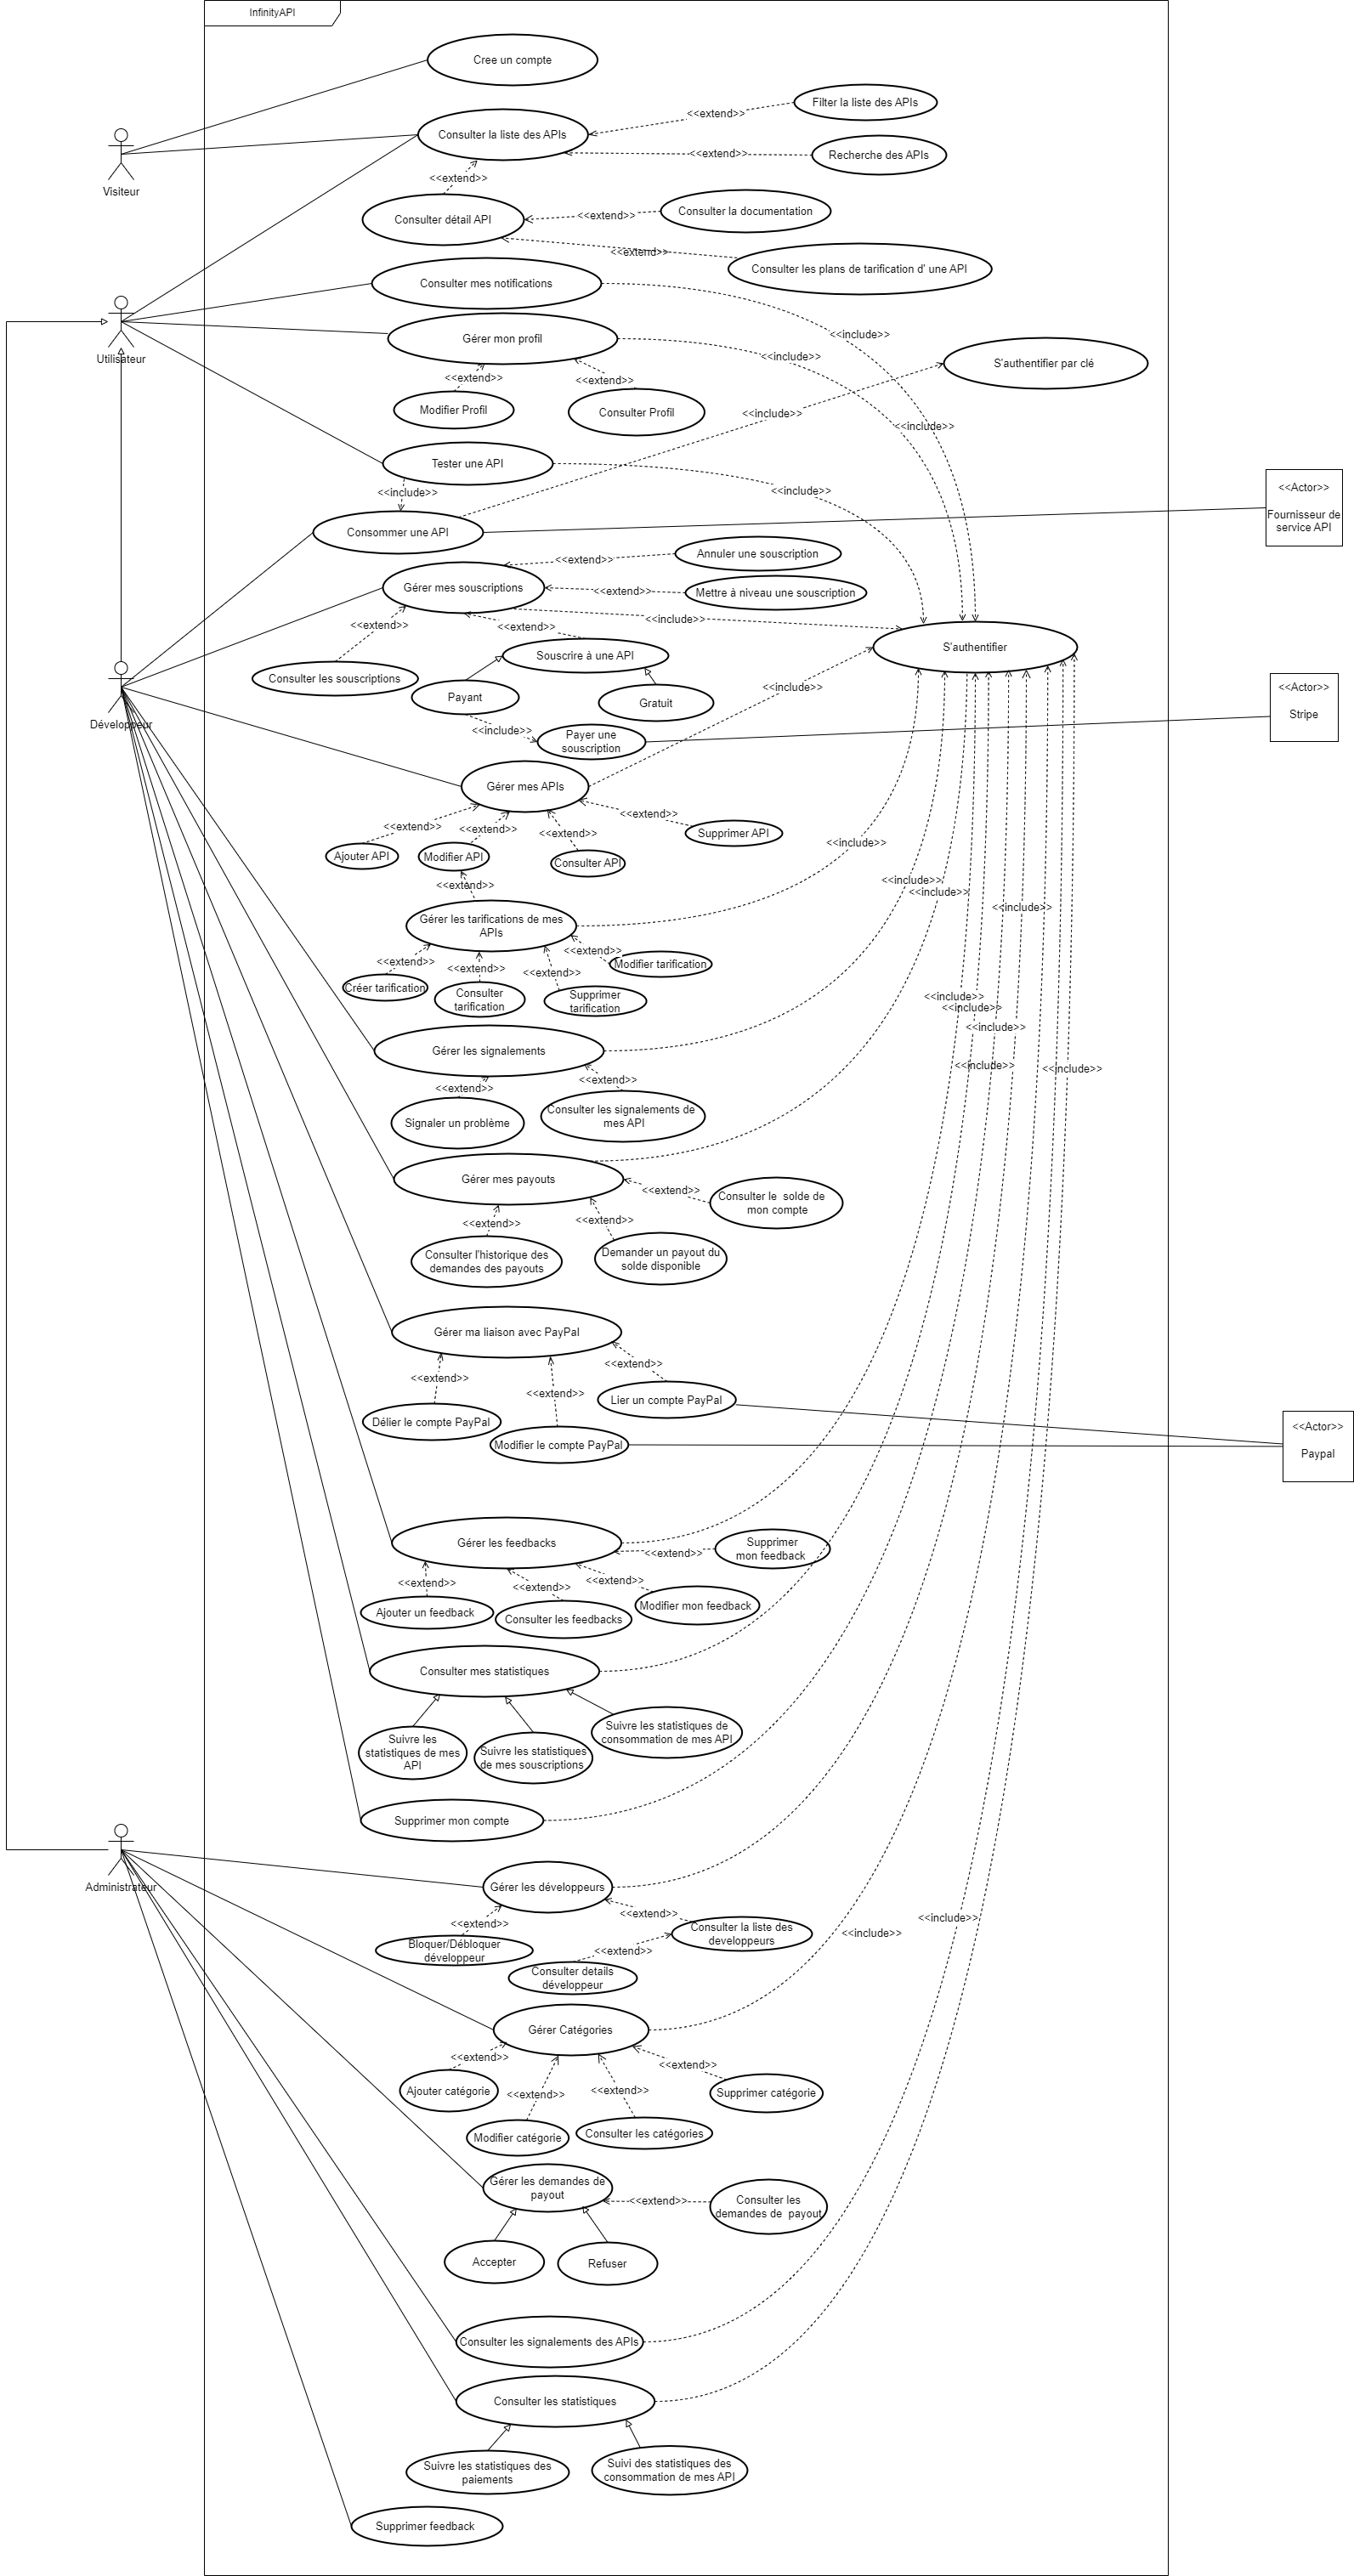
\includegraphics[width=0.6\columnwidth]{usecaseglobale.png }}
    {\\\textbf{Figure annexe 1.1:} Diagramme de cas d'utilisation globale}
\end{figure}


\subsection{La représentation NoSQL associée à la base de données de la MarketPlace d’API}

\addcontentsline{lof}{figure}{Annexe 1.2 La représentation NoSQL associée à la base de données }
\begin{figure}[H]
    \centering
    \frame{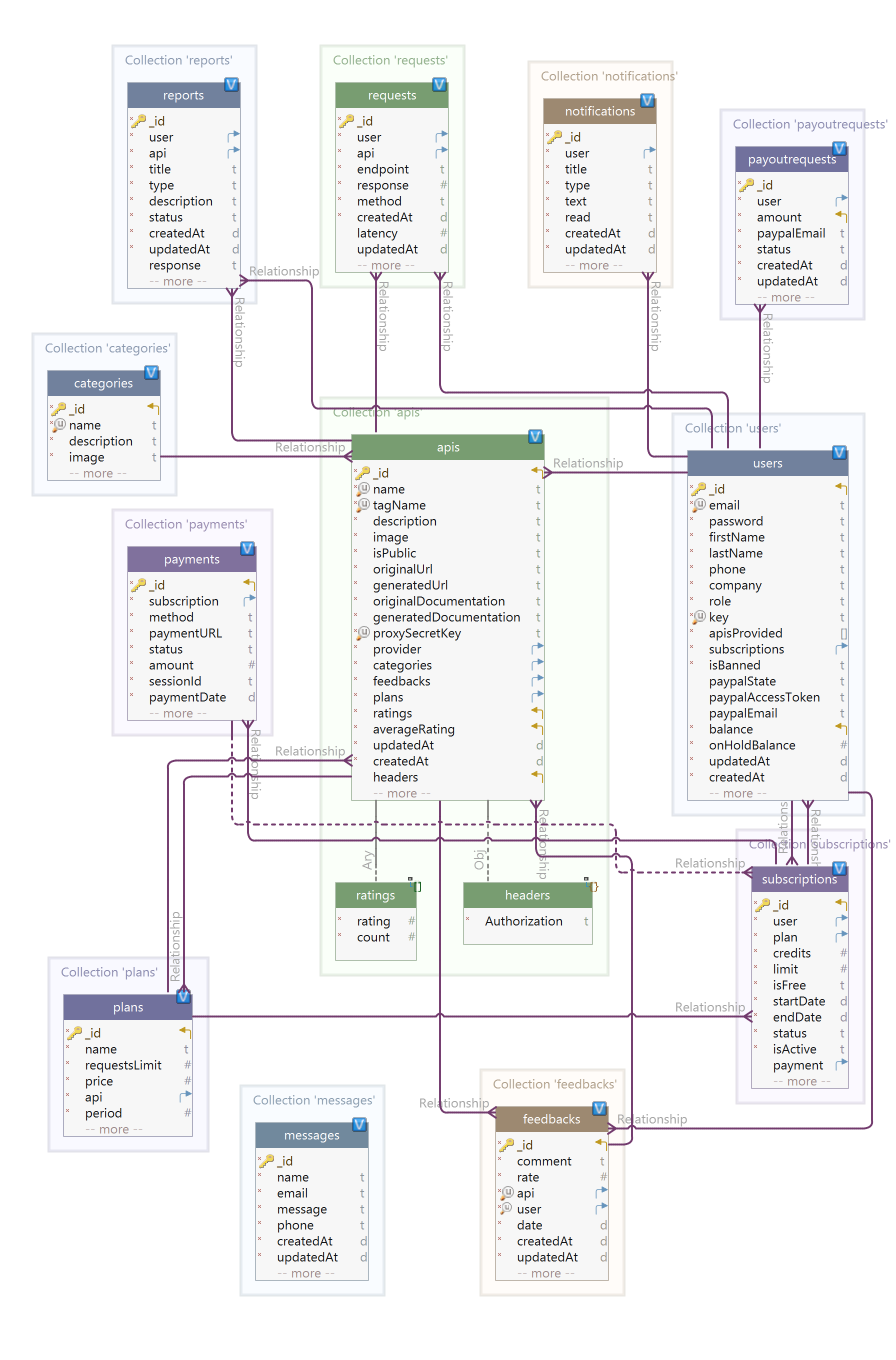
\includegraphics[width=0.8\columnwidth]{db s3.png }}
    {\\\textbf{Figure annexe 1.2:} La représentation NoSQL associée à la base de données }
\end{figure}




 \subsection{Diagramme de séquence "Authentification"}
 Ce diagramme de séquence illustre la séquence d'interactions entre les différents composants de la marketplace pour  l'authentification. Le développeur commence par remplir le formulaire \sloppy d'authentification. Si les champs sont invalides, un message d'erreur est affiché. Sinon, une requête HTTP est envoyée au backend. Le backend vérifie ensuite si les données fournies existent et si elles proviennent d'une page précédente. Si elles proviennent d'une page précédente, il retourne une réponse positive. Sinon, il redirige l'utilisateur vers la page d'accueil. En cas de données invalides, un message d'erreur est affiché.
 \addcontentsline{lof}{figure}{Annexe 1.3 Diagramme de séquence "Authentification"}
 \begin{figure}[H]
    \centering
    \frame{\includegraphics[width=1.1\columnwidth]{Diagramme_de_séquence_Authentification.jpg}}
    {\\\textbf{Figure annexe 1.3:} Diagramme de séquence "Authentification"}
    \label{fig:logo_tt}
\end{figure}
\pagebreak


\subsection{Diagramme de séquence "statistique des souscriptions d'un développeur"}
Le diagramme de séquence illustre les interactions entre les différents composants de la marketplace pour consulter les statistiques de consommation d'une API. \\
Lorsqu'un développeur consulte le tableau de bord des statistiques pour le graphique de souscription, une requête HTTP est envoyée au backend. Le backend vérifie alors la validité du jeton au niveau du middleware d'authentification. Si le jeton est invalide, un message d'erreur "jeton non valide" est renvoyé. Sinon, le backend exécute la fonction 'getConsumerAnalytics au niveau du contrôleur', qui retourne les données statistiques. Ces données sont ensuite envoyées au service du front-end, puis au contrôleur, et elles sont affichées au niveau du graphique de souscription. 
\addcontentsline{lof}{figure}{Annexe 1.4 Diagramme de séquence "Statistique des souscriptions"}
\begin{figure}[H]
    \centering
    \frame{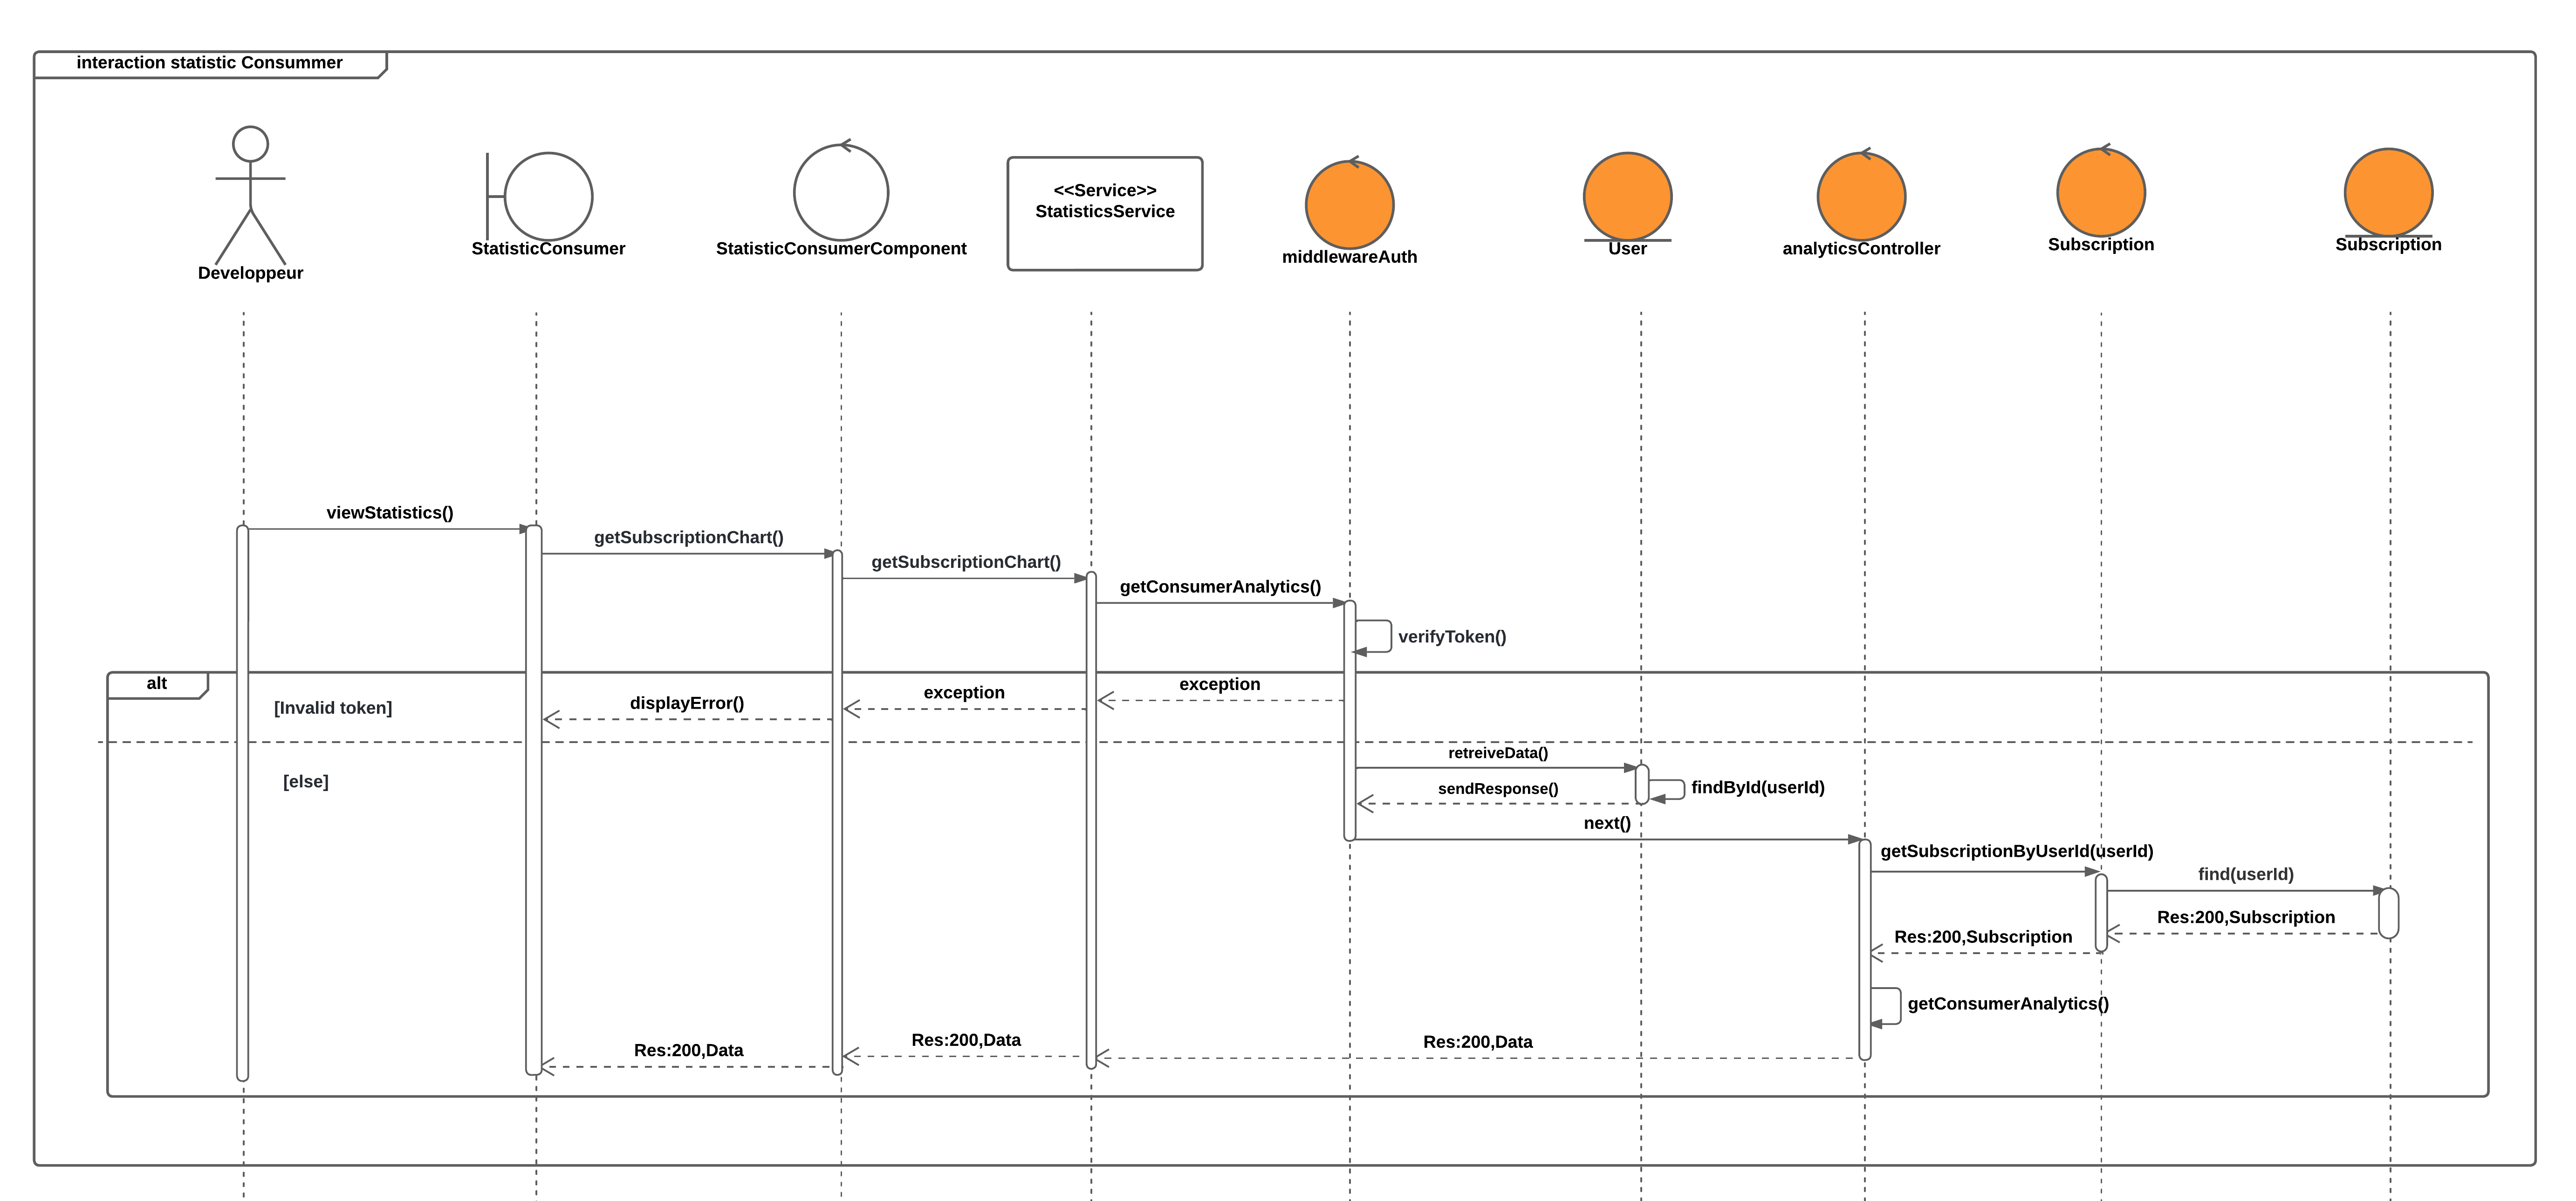
\includegraphics[width=1\columnwidth]{diagrammedesequencestatistiquesubscription.png    }}
    {\\\textbf{Figure annexe 1.4:}Diagramme de séquence "Statistique des souscriptions"    }
    \label{fig:logo_tt}
\end{figure}
 \pagebreak
%\addcontentsline{toc}{section}{Annexe 1.~Exemple d'annexe}

%Les chapitres doivent présenter l’essentiel du travail. Certaines informations-trop  détaillées  ou constituant un complément d’information pour toute personne qui désire mieux comprendre ou refaire une expérience décrite dans le document- peuvent être mises au niveau des annexes. Les annexes, {\bf placées après la bibliographie}, doivent donc être numérotées avec des titres (Annexe1, Annexe2, etc.).

%\addcontentsline{lot}{table}{Annexe 1.1~~~Exemple tableau dans l'annexe}

%Le tableau annexe 1.1 présente un exemple d'un tableau dans l'annexe.

%{\raggedright \textbf{Tableau annexe 1.1:}~Exemple tableau dans l'annexe}


\newpage
%===================== ANNEXE 2 =====================%
\section{Annexe 2: Complément d'interfaces graphiques}

\addcontentsline{lof}{figure}{Annexe 2.1 Interface de liste des APIs d'un développeur }
Cette interface présente la page de la liste des APIs du développeur 
\begin{figure}[H]
    \centering
    \frame{\includegraphics[width=0.9\columnwidth]{ Interface_de_liste_des_APIs_dun_développeur.png   }}
    {\\\textbf{Figure annexe 2.1:}Interface de liste des APIs d'un développeur }
    \label{fig:logo_tt}
\end{figure}


\addcontentsline{lof}{figure}{Annexe 2.2 Interface de statistique des API dans le marketplace}
Cette interface représente les statistiques des nouvelles API intégrées dans la marketplace pour l'année en cours, y compris un graphique montrant le nombre d'API disponibles pour chaque catégorie.
\begin{figure}[H]
    \centering
    \frame{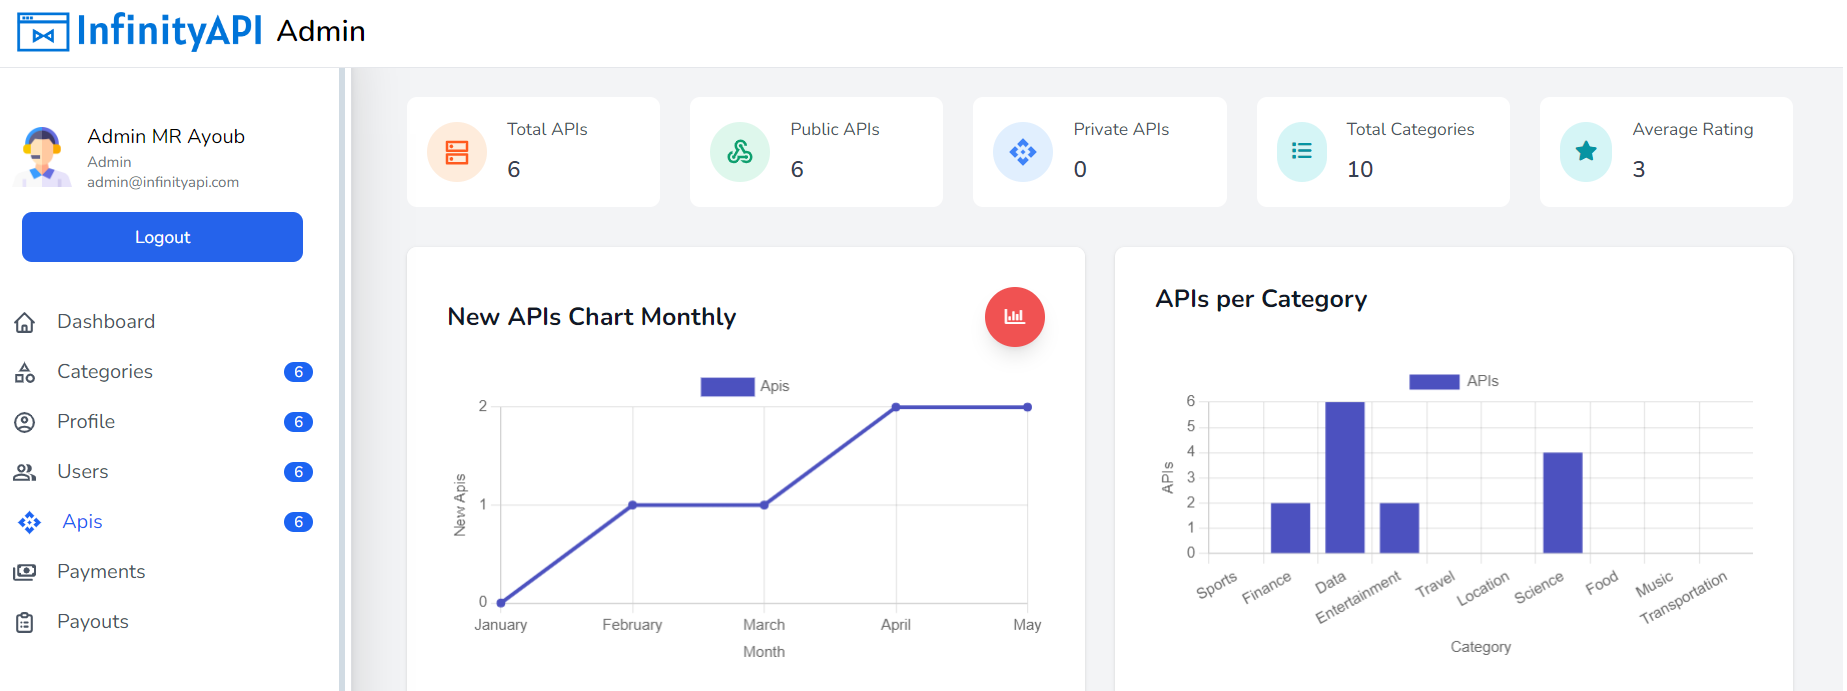
\includegraphics[width=1.1\columnwidth]{    interfacedestatistiquedesApidanslemarketplace.png }}
    {\\\textbf{Figure annexe 2.2:}Interface du provider d'API }
    \label{fig:logo_tt}
\end{figure}


\addcontentsline{lof}{figure}{Annexe 2.3 Interface de statistique du consommateur d'API}
Cette interface représente les statistiques des consommateurs sur les souscriptions aux API, ainsi que les statistiques des requêtes effectuées et les statistiques de latence moyenne des API.
\begin{figure}[H]
    \centering
    \frame{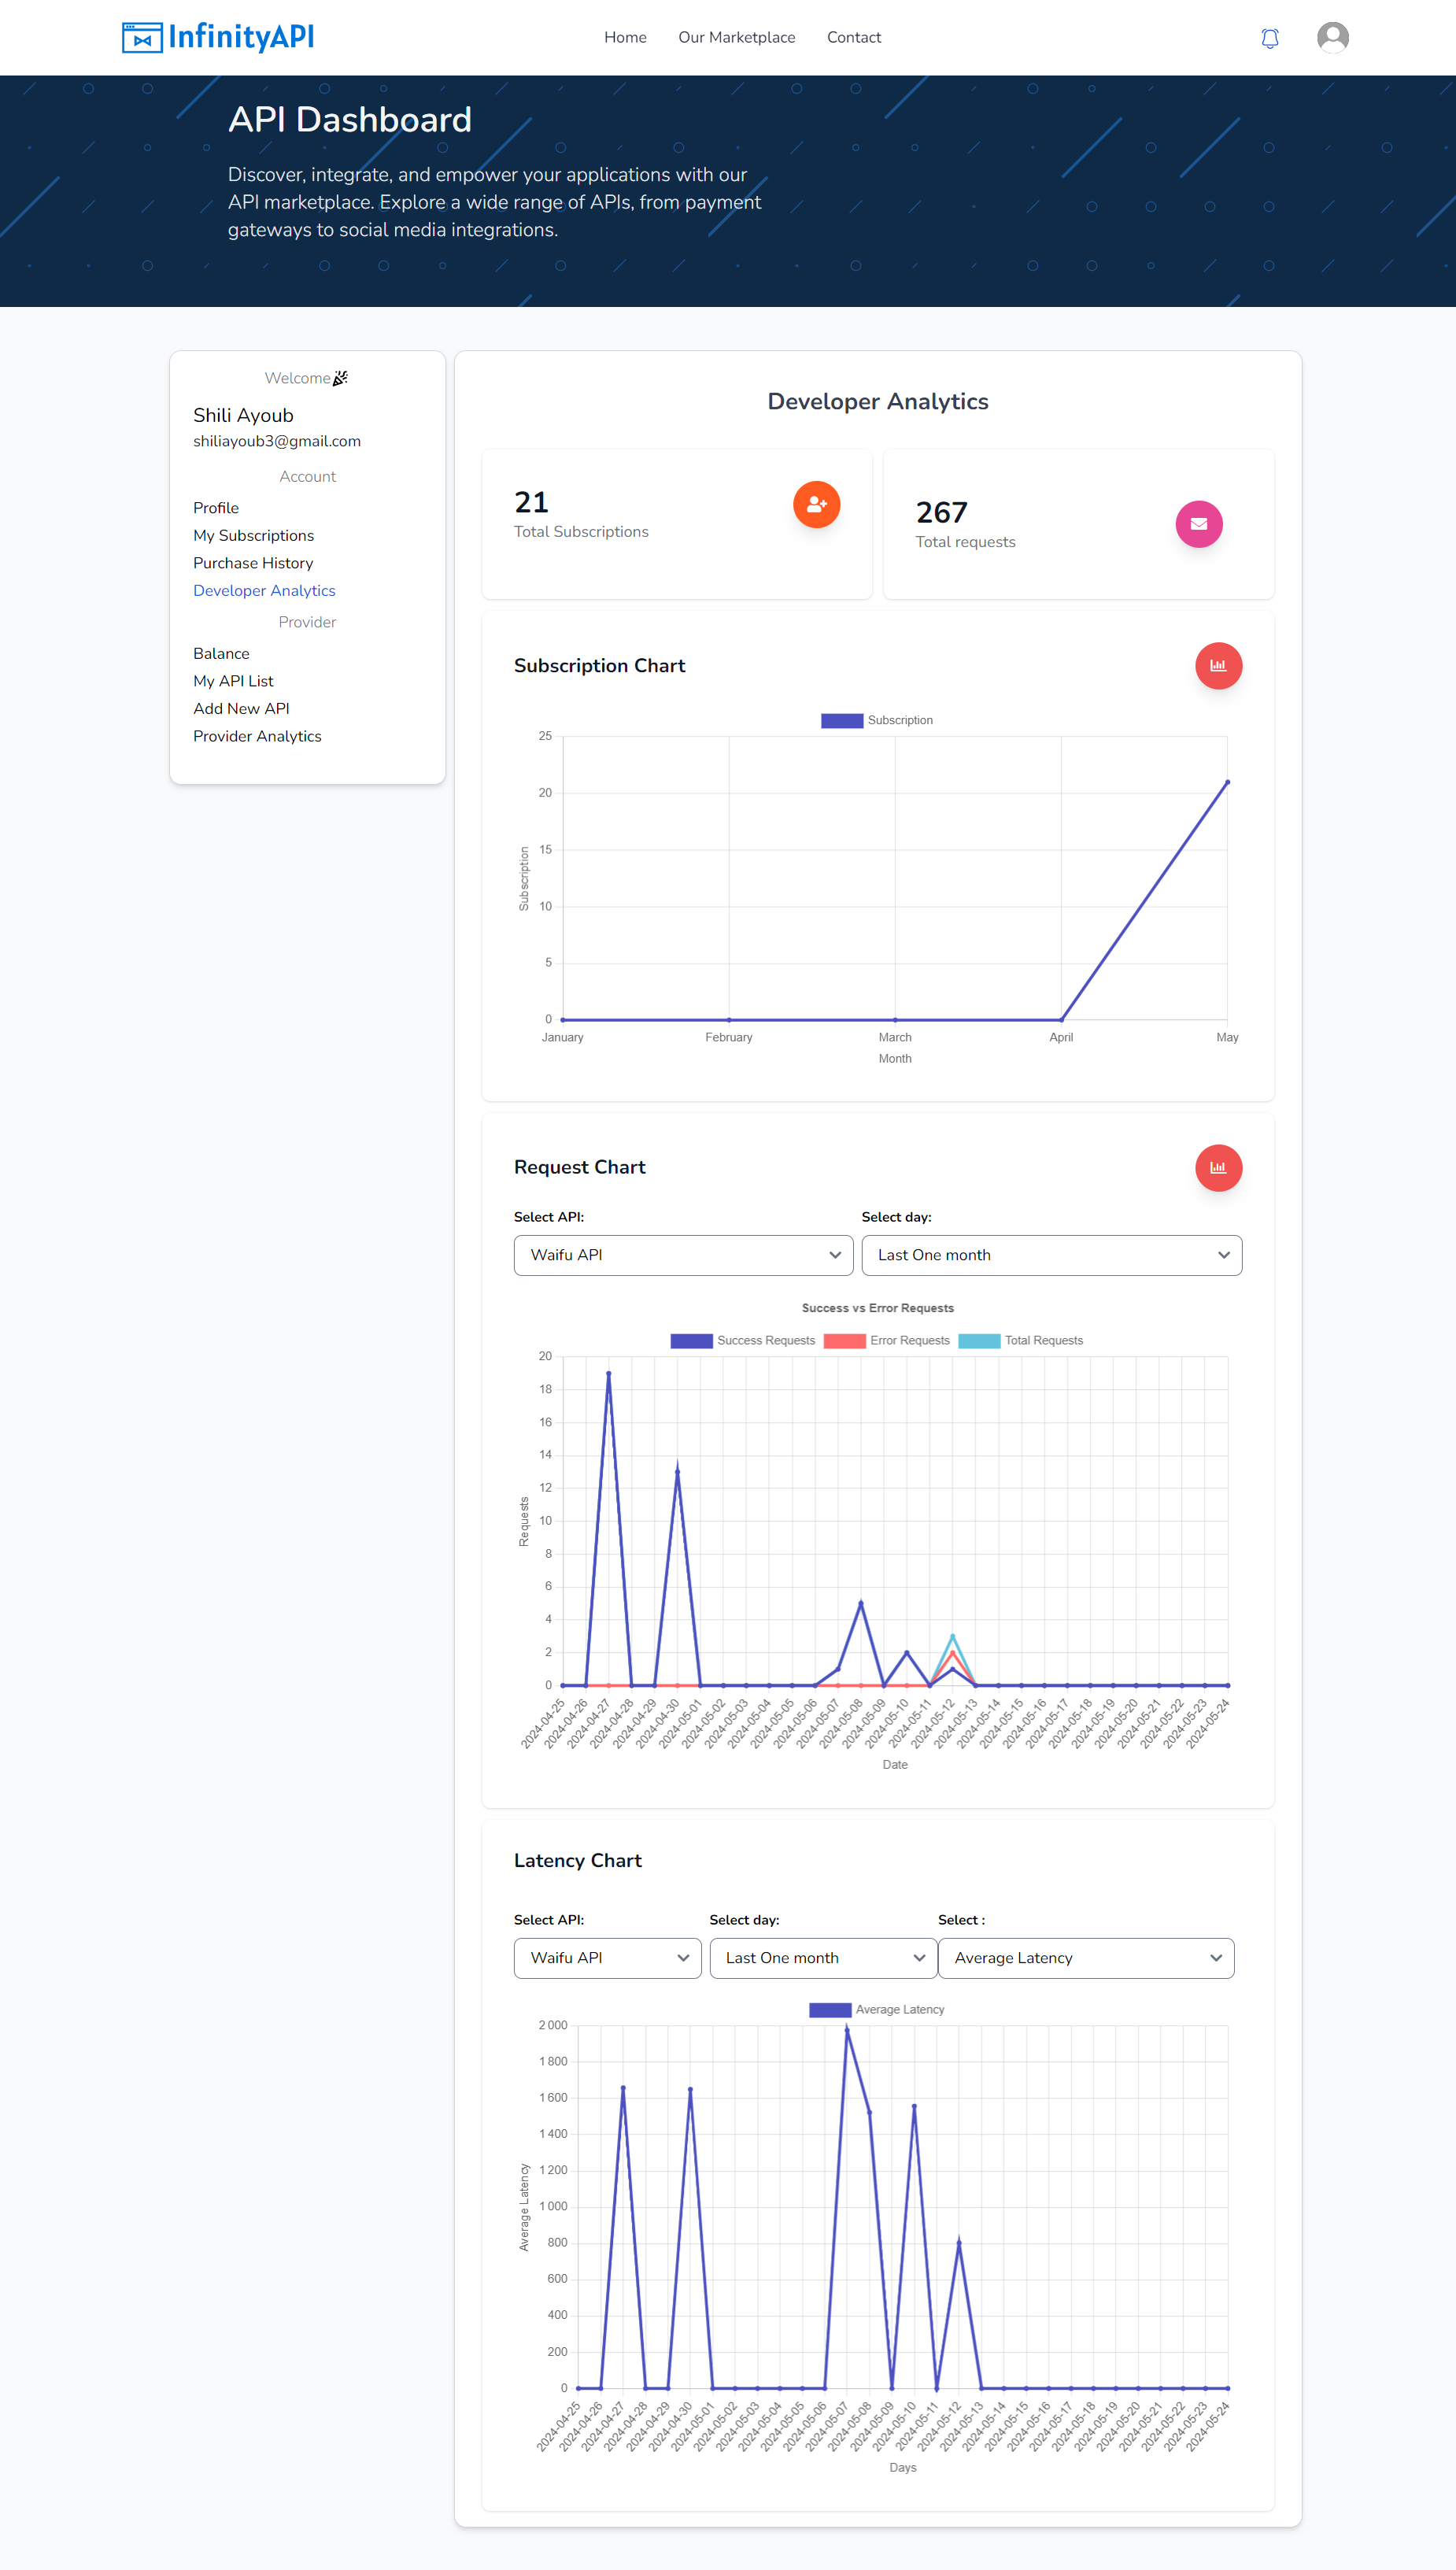
\includegraphics[width=0.75\columnwidth]{interfaceConsumerLineChart.png}}
    {\\\textbf{Figure annexe 2.3:}Interface de statistique du consommateur d'API }
    \label{fig:logo_tt}
\end{figure}

\addcontentsline{lof}{figure}{Annexe 2.4 Interface de statistique du consommateur d'API}
Cette interface présente deux graphiques : l’un affichant les demandes de payouts effectués dans la marketplace par mois, et l’autre montrant le statut des demandes de payout realisée dans la marketplace. 
\begin{figure}[H]
    \centering
    \frame{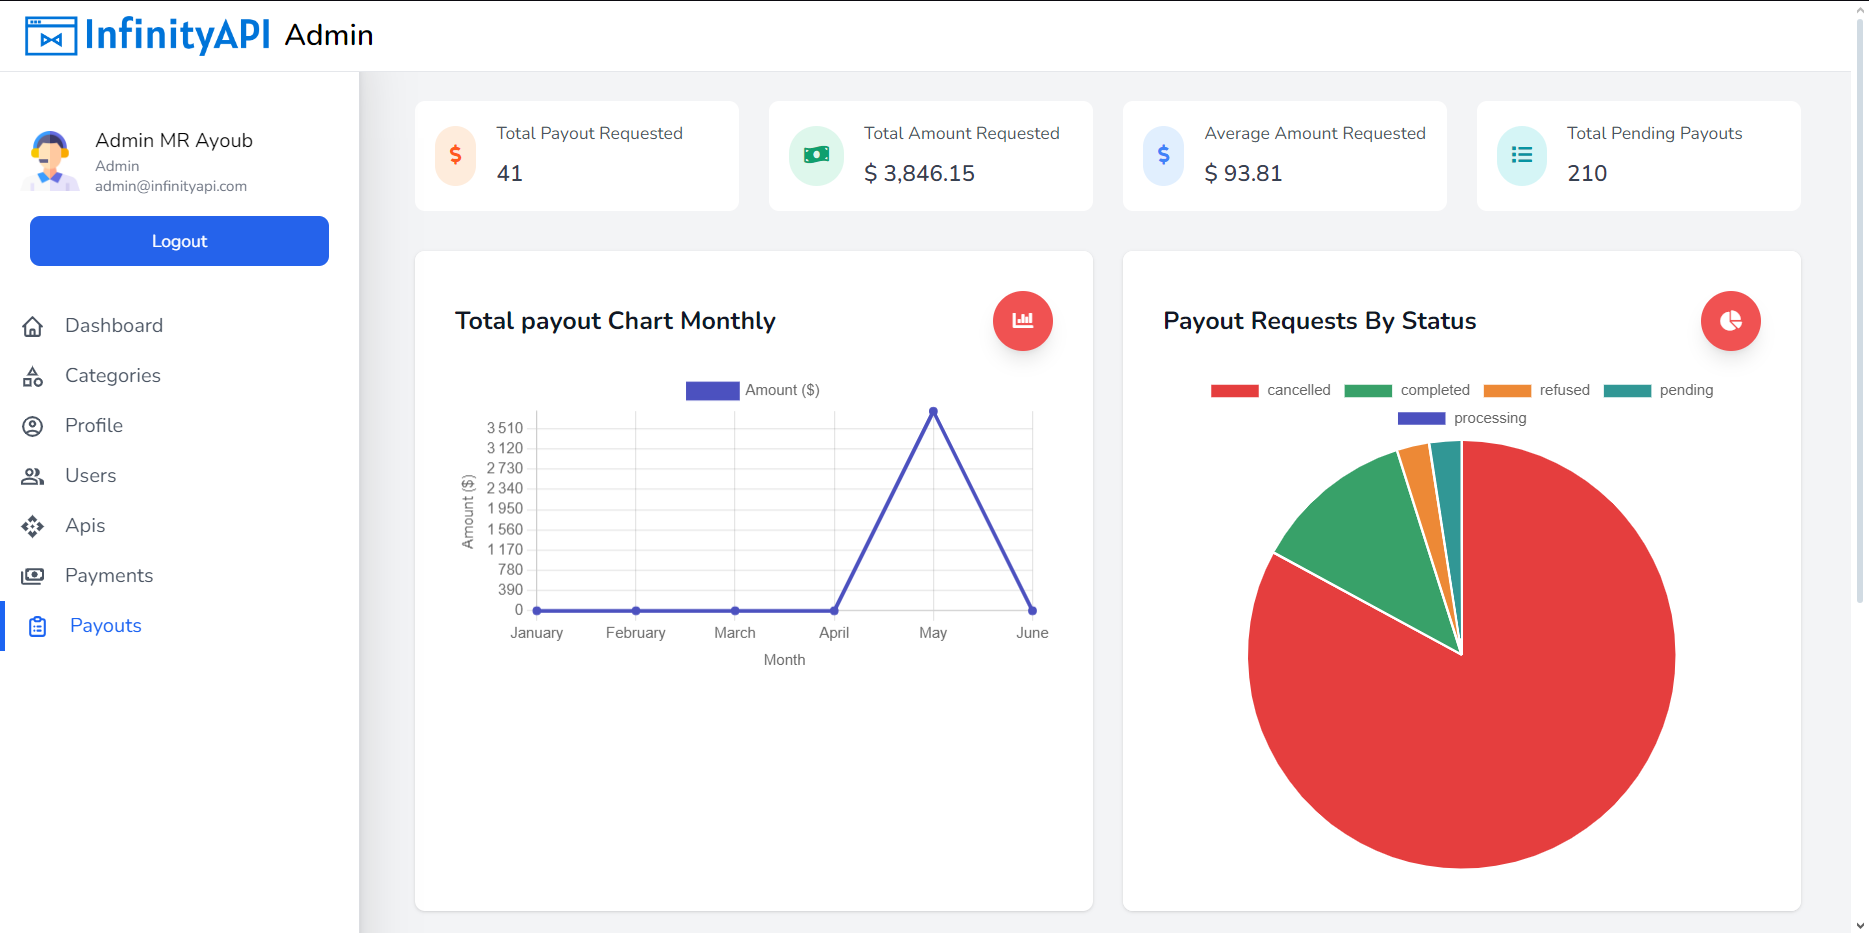
\includegraphics[width=1\columnwidth]{  interfacedespayoutrealiserdanslemarketplace.png}}
    {\\\textbf{Figure annexe 2.4:}Interface des statistique des demandes de payout }
    \label{fig:logo_tt}
\end{figure}
\pagebreak



